\documentclass{beamer}
\usetheme{Madrid}
%Information to be included in the title page:
\title{Effektive Zombies}
\author{Martin Ilgner}
\institute{University of Tübingen}
\date{Project for the Effective Programming with Effects Course, WS 24/25}

\usepackage{tikz-uml} %UML

\setlength{\abovecaptionskip}{0pt plus 3pt minus 2pt}

\begin{document}
	\setbeamertemplate{caption}{\raggedright\insertcaption\par}
	\setbeamertemplate{itemize item}{\raisebox{0.1em}{\textbullet}} % Adjust bullet position
	%Presentation requirements: 
	%Duration: 8-10 minutes for presentation, 2-3 minutes for questions
	%Content should include:
	%1. Motivation for your technical problem,
	%2. technical challenges you encountered and overcame,
	%3. specific focus on how you used Effekt's unique features (effects and handlers), and
	%4. live demonstration of your software
	
	%1. Was ist es grob
	%2. Warum?
	%3. Wie ist es aufgebaut:
	%	- FFI
	%	- Data structures
	%	- Data flow   (where effects?)
	%4. Demo
	% Was für Challenges
	
	%Bis Freitag Abend Präsentation fertig, dann üben
	%falls noch Zeit: noch kurz background machen + zombie pixel line fixen
	
	\frame{\titlepage}
	
	\begin{frame}
		\frametitle{What is it?}
		\begin{Large}
		\begin{itemize}
			\setlength{\itemsep}{.5em}
			\item Browser Game $\rightarrow$ js-web backend
			\item Top Down 
			\item Survival
			%image of game
		\end{itemize}
		\end{Large}
	\end{frame}
	
	\begin{frame}
		\frametitle{''Motivation for your technical problem''}
		\begin{Large}
		\begin{itemize}
			\setlength{\itemsep}{1em}
			\item Everybody likes games
			\item Canvas API
		\end{itemize}
		\end{Large}
	\end{frame}
	
	\begin{frame}[plain, c]
		\begin{center}
			\Huge Demo
		\end{center}
	\end{frame}
	
	\begin{frame}
		\frametitle{Rough Structure}
		\begin{Large}
		\begin{itemize}
			\setlength{\itemsep}{.5em}
			\item Game loop as idleCallback: update, render
			\item Event listeners for user input
			\item Gamestate
		\end{itemize}
		\end{Large}
	\end{frame}
	
	\begin{frame}
		\frametitle{Gamestate}
		\begin{center}
		\scalebox{.59}{
		\begin{tikzpicture}
			\umlclass[x = 8, y = 1, width = 250]{GameState}{
				player: Player \\
				objects: List[GameObject] \\
				timers: GameTimer \\
				wave: Int \\
				score: Score \\
				menu: Menu
			}{}
			\umlclass[x = -1, y = 0]{Player}{
				drawable: SimpleDrawable \\
				gun: SimpleDrawable \\
				health: Int \\
				speed: Double
			}{}
			\umlenum[x = 2, y = -4]{GameObject}{
				Bullet(ManipulatedDrawable, Vec2d) \\
				Zombie(ManipulatedDrawable, Vec2d, LifeState)	
			}{}
			\umlclass[x = 9, y = -3]{GameTimer}{
				zombieTimer: Timer \\
				waveTimer: Timer \\
				bulletTimer: Timer
			}{}
			\umlclass[x = 16, y = 0]{Score}{
				score: Int \\
				combo: Int \\
				maxCombo: Int
			}{}
			\umlenum[x = 14, y = -4]{Menu}{
				Main \\
				InGame \\
				Retry
			}{}
			\umlenum[x = 4.8, y = -7.5]{LifeState}{
				Dead \\
				Alive
			}{}
			\umlclass[x = 9, y = -6.5]{Timer}{left: Int}{}
			\umlcompo[geometry=-|, anchor1=168]{GameState}{Player}
			\umlcompo[geometry=-|, anchor1=173]{GameState}{GameObject}
			\umlcompo[geometry=-|-, anchor1=178, anchor2=160, arm1=-1cm]{GameState}{GameTimer}
			\umlcompo[anchor1=-10, geometry=-|]{GameState}{Score}
			\umlcompo[anchor1=-15, geometry=-|]{GameState}{Menu}
			\umlcompo[geometry=--, anchor1=-25]{GameObject}{LifeState}
			\umlcompo{GameTimer}{Timer}
		\end{tikzpicture}}
		\end{center}
	\end{frame}
	
	\begin{frame}
		\frametitle{Update}
		\begin{Large}
		\begin{enumerate}
			\item Check "Menu"
			\item Spawn Bullets/Zombies
			\item Collision checks
			\item Move objects and player
			\item Update timers/score/wave
			\item Repeat
		\end{enumerate}
		\end{Large}
	\end{frame}
	
	\begin{frame}
		\frametitle{FFI}
		\begin{columns}
			\begin{column}{.5\linewidth}
			\begin{itemize}
				\item talking to Canvas API:
				\begin{itemize}
					\item createCanvas
					\item drawImage, drawRect, ...
					\item set/getTransformation
					\item clear
				\end{itemize}
				\item Callbacks and Event(listeners)
				\item Time
				\item Window Size
			\end{itemize}
			\end{column}
			\begin{column}{.5\linewidth}
				\begin{figure}
					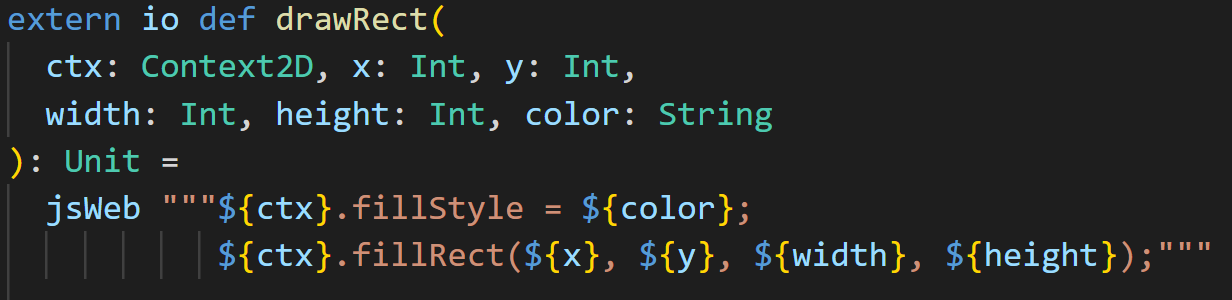
\includegraphics[width=\linewidth]{images/drawRect.png}
				\end{figure}
				\begin{figure}
					\includegraphics[width=\linewidth]{images/getKeygetClient.png}
				\end{figure}
				\begin{figure}
					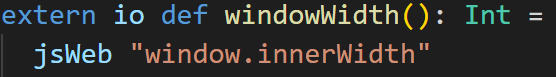
\includegraphics[width=\linewidth]{images/getWindowWidth.png}
				\end{figure}
			\end{column}
		\end{columns}
	\end{frame}
	
	\begin{frame}
		\frametitle{Use of Effects}
		\begin{Large}
		\begin{itemize}
			\setlength{\itemsep}{1em}
			\item random
			\item elapsed
			\item animationFinished
			\item Canvas
			\item Input
		\end{itemize}
		\end{Large}
	\end{frame}

	\begin{frame}
		\frametitle{animationFinished}
		\begin{figure}
			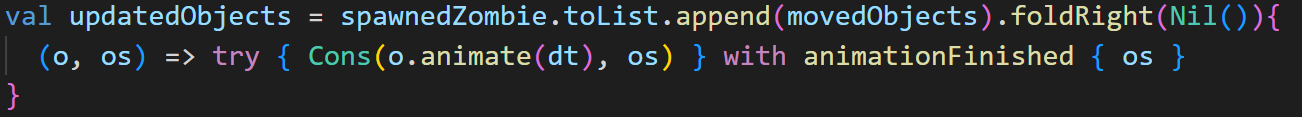
\includegraphics[width=.75\linewidth]{images/animate1.png}
			\caption{game/game.effekt}
		\end{figure}
		\begin{figure}
			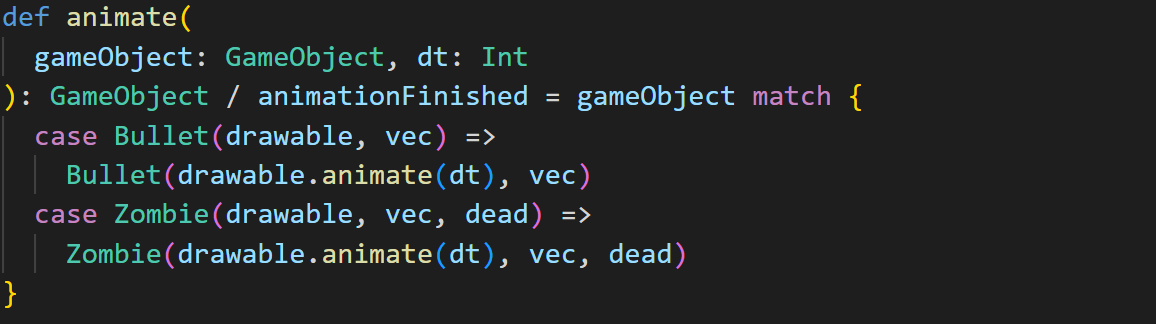
\includegraphics[width=.75\linewidth]{images/animate2.png}
			\caption{game/gameobject.effekt}
		\end{figure}
		\begin{figure}
			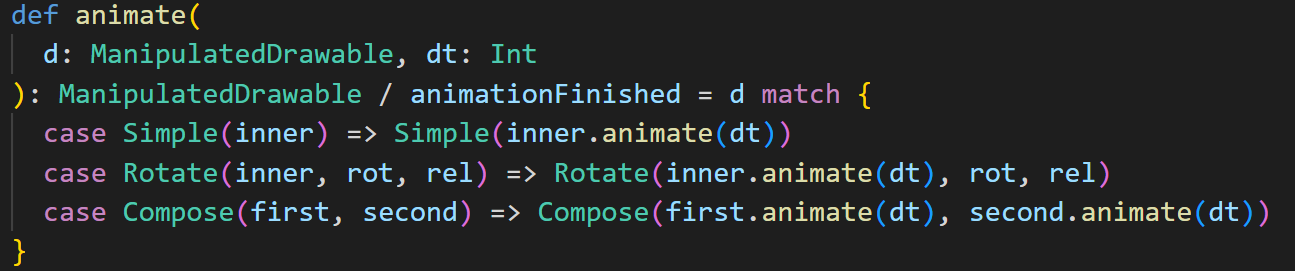
\includegraphics[width=.75\linewidth]{images/animate3.png}
			\caption{drawable/manipulated.effekt}
		\end{figure}
	\end{frame}
	
	\begin{frame}
		\frametitle{animationFinished}
		\begin{figure}
			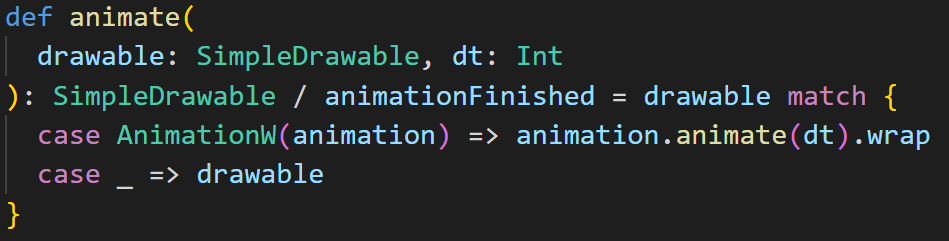
\includegraphics[width=.9\linewidth]{images/animate4.png}
			\caption{drawable/simple.effekt}
		\end{figure}
		\begin{figure}
			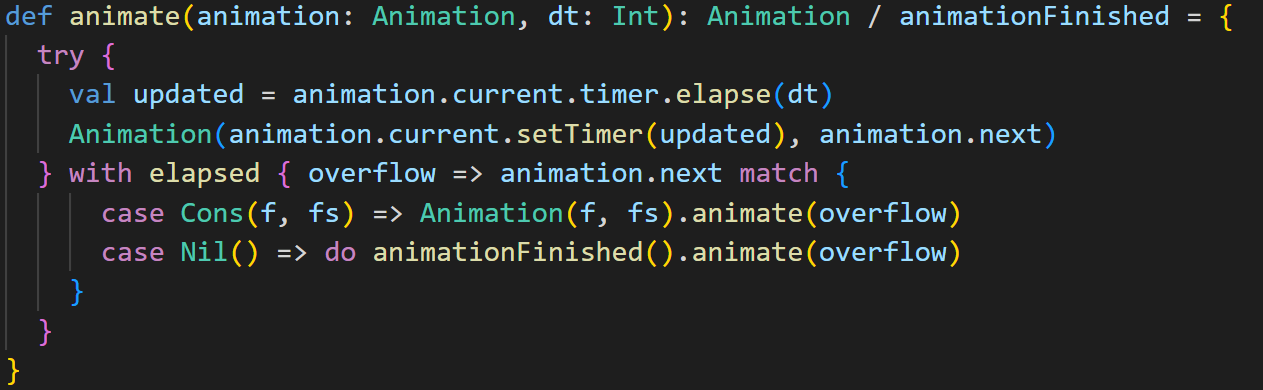
\includegraphics[width=.9\linewidth]{images/animate5.png}
			\caption{drawable/simple.effekt}
		\end{figure}
	\end{frame}
	
	
	\begin{frame}
		\frametitle{Challenges}
		\begin{Large}
		\begin{itemize}
			\setlength{\itemsep}{.8em}
			\item Collision
			\item Resizing
			\item Key drops $\rightarrow$ intervals
		\end{itemize}
		\end{Large}
	\end{frame}
	
	\begin{frame}[plain, c]
		\begin{center}
		\begin{Huge}
			Questions?
		\end{Huge}
		\end{center}
	\end{frame}
	
	
	
	
	
	
	
	
	
	
		%Delete this slide?
	\iffalse
	\begin{frame}
		\frametitle{Drawables}
		\begin{center}
			\scalebox{.55}{
				\begin{tikzpicture}
					\umlenum{ManipulatedDrawable}{
						Simple(SimpleDrawable) \\
						Rotate(inner: ManipulatedDrawable, rotation: Double, relativeTo: Option[Vec2d]) \\
						Compose(ManipulatedDrawable, ManipulatedDrawable)
					}{}
					\umlenum[x = -7, y = -5]{SimpleDrawable}{
						Rect(upperLeft: Vec2d, width: Double, height: Double, Color) \\
						Circle(center: Vec2d, radius: Double, Color) \\
						Image(name: String, src: Option[Drawable], dest: Drawable, hitbox: Hitbox) \\
						Animation(current: Frame, next: List[Frame])
					}{}
					\umlenum[x = 6, y = -5]{Hitbox}{
						HRect(Vec2d, Vec2d, Vec2d, Vec2d) \\
						HCircle(center: Vec2d, radius: Double) \\
						HCompose(Hitbox, Hitbox)
					}{}
					\umlclass[x = -10, y = 0]{Text}{
						text: String \\
						position: Vec2d \\
						fontSizePX: Int \\
						...
					}{}
					\umlclass[x = -7, y = -9]{Frame}{
						frame: SimpleDrawable \\
						timer: Timer
					}{}
					\umlcompo[anchor1=179, geometry=-|]{ManipulatedDrawable}{SimpleDrawable}
					\umlcompo[anchor1=-5, geometry=-|]{SimpleDrawable}{Hitbox}
					\umluniassoc[arg1=transformable to, pos1=.5]{ManipulatedDrawable}{Hitbox}
					\umluniassoc[arg1=transformable to, pos1=.5]{SimpleDrawable}{Hitbox}
					\umlcompo[anchor1=-90]{SimpleDrawable}{Frame}
			\end{tikzpicture}}
		\end{center}
	\end{frame}
	\fi
	
\end{document}